\section{Appendix}

\subsection{Community labels of super-vertices}

We also attempt two different variations of Parallel Leiden algorithm, one where the community labels of super-vertices (upon aggregation) is based on the local-moving phase (\textit{move-based}), and the other where the community labels of super-vertices is based on the refinement phase (\textit{refine-based}). Our observations indicate that both approaches have roughly the same runtime and modularity on average, as indicated by Figures \ref{fig:leidenreopt-runtime} and \ref{fig:leidenreopt-modularity}. Accordingly, we stick to the move-based approach, which is the one recommended by Traag et al. \cite{com-traag19}. However, refine-based approach may be more suitable for the design of dynamic Leiden algorithm (for dynamic graphs).

\begin{figure}[hbtp]
  \centering
  \subfigure{
    \label{fig:leidenreopt-runtime--all}
    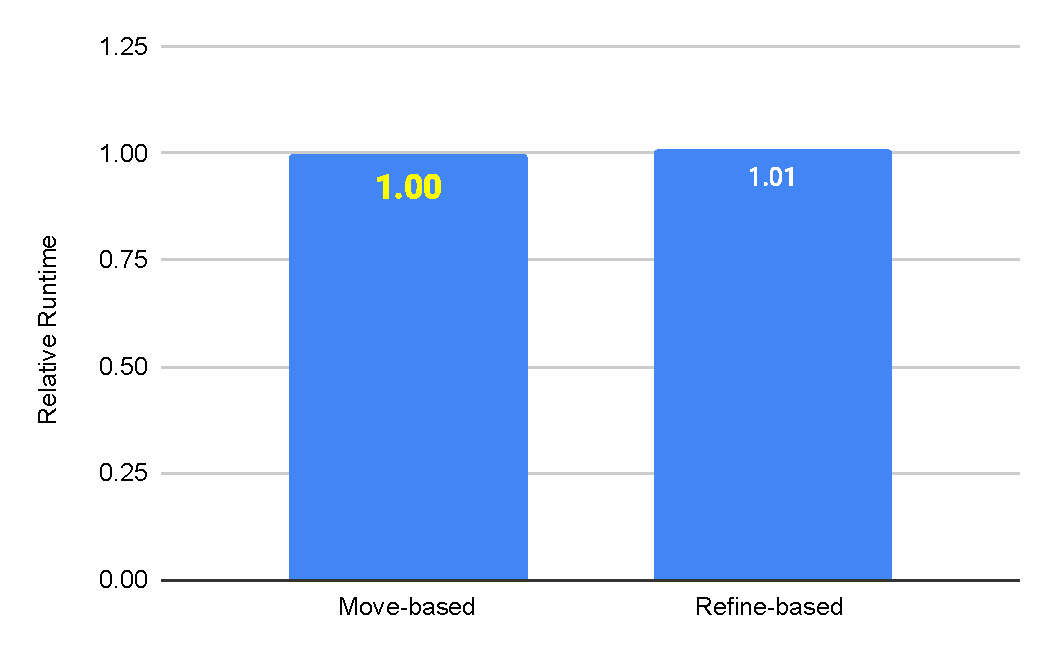
\includegraphics[width=0.98\linewidth]{out/leidenreopt-runtime.pdf}
  } \\[-2ex]
  \caption{Average relative runtime for \textit{move-based} and \textit{refine-based} communities for super-vertices upon aggregation with parallel Leiden algorithm, for all graphs in the dataset.}
  \label{fig:leidenreopt-runtime}
\end{figure}

\begin{figure}[hbtp]
  \centering
  \subfigure{
    \label{fig:leidenreopt-modularity--all}
    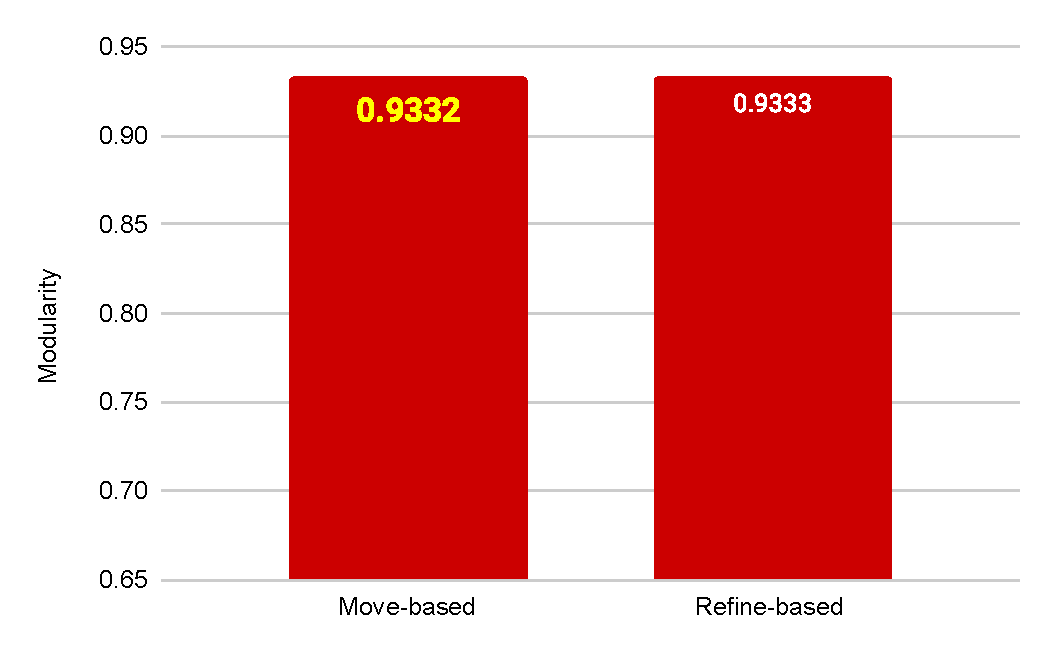
\includegraphics[width=0.98\linewidth]{out/leidenreopt-modularity.pdf}
  } \\[-2ex]
  \caption{Average modularity for \textit{move-based} and \textit{refine-based} communities for super-vertices upon aggregation with parallel Leiden algorithm, for all graphs in the dataset.}
  \label{fig:leidenreopt-modularity}
\end{figure}

